% slides discussing the invariant manifolds and introducing poincare sections
\section*{}
\subsection*{Invariant Manifolds}

\begin{frame}%--------------------------------------------%
\frametitle{Invariant Manifolds}
\begin{itemize}
	\item Tube structure governs orbital motion
	\item \textcolor{green}{Stable}/\textcolor{red}{Unstable} `tubes' divide orbits
	\item Poincar\'e section visualizes intersection
\end{itemize}
 \begin{figure}
     \centering
     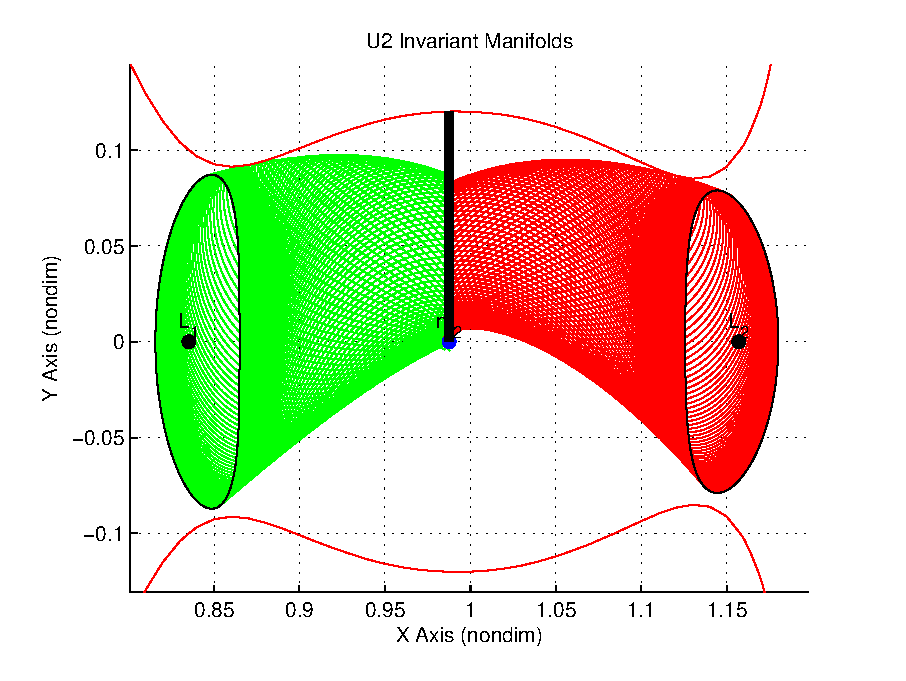
\includegraphics[width=0.5\columnwidth]{U2_Manifolds}%
     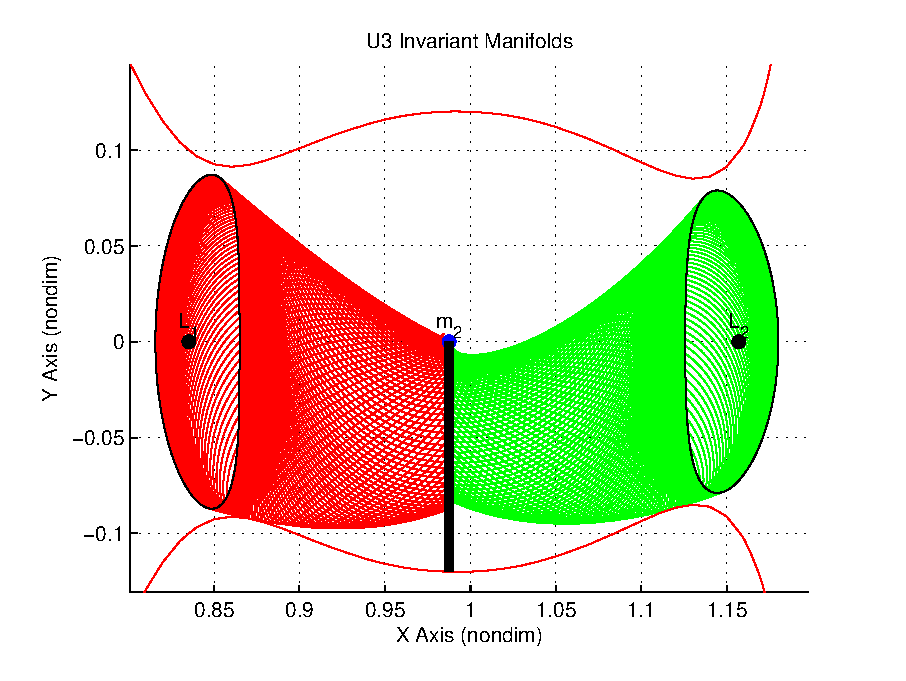
\includegraphics[width=0.5\columnwidth]{U3_Manifolds}
\end{figure}

	\note[itemize]{
		\item Manifolds asymptotically depart/arrive at periodic orbit
	}
\end{frame}%--------------------------------------------%

\begin{frame}[t]%---------------------------------------%
\frametitle{Poincar\'e Section}
	\begin{itemize}
		\item Define hyperplane transverse to dynamic flow
		\item Analysis on a lower dimensional space
	\end{itemize}
 \begin{figure}
     \centering
     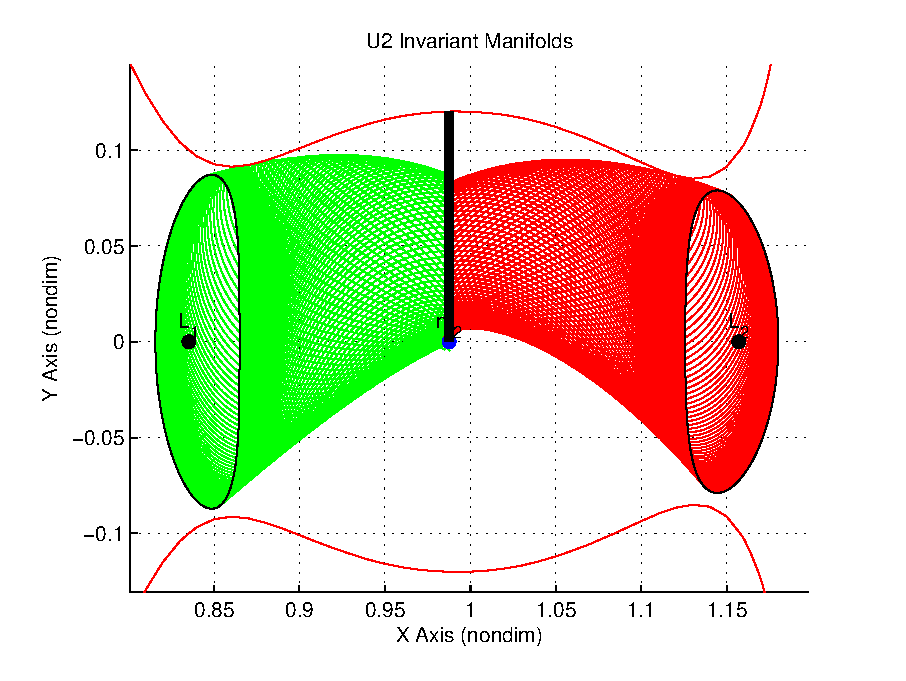
\includegraphics[width=0.5\columnwidth]{U2_Manifolds}%
     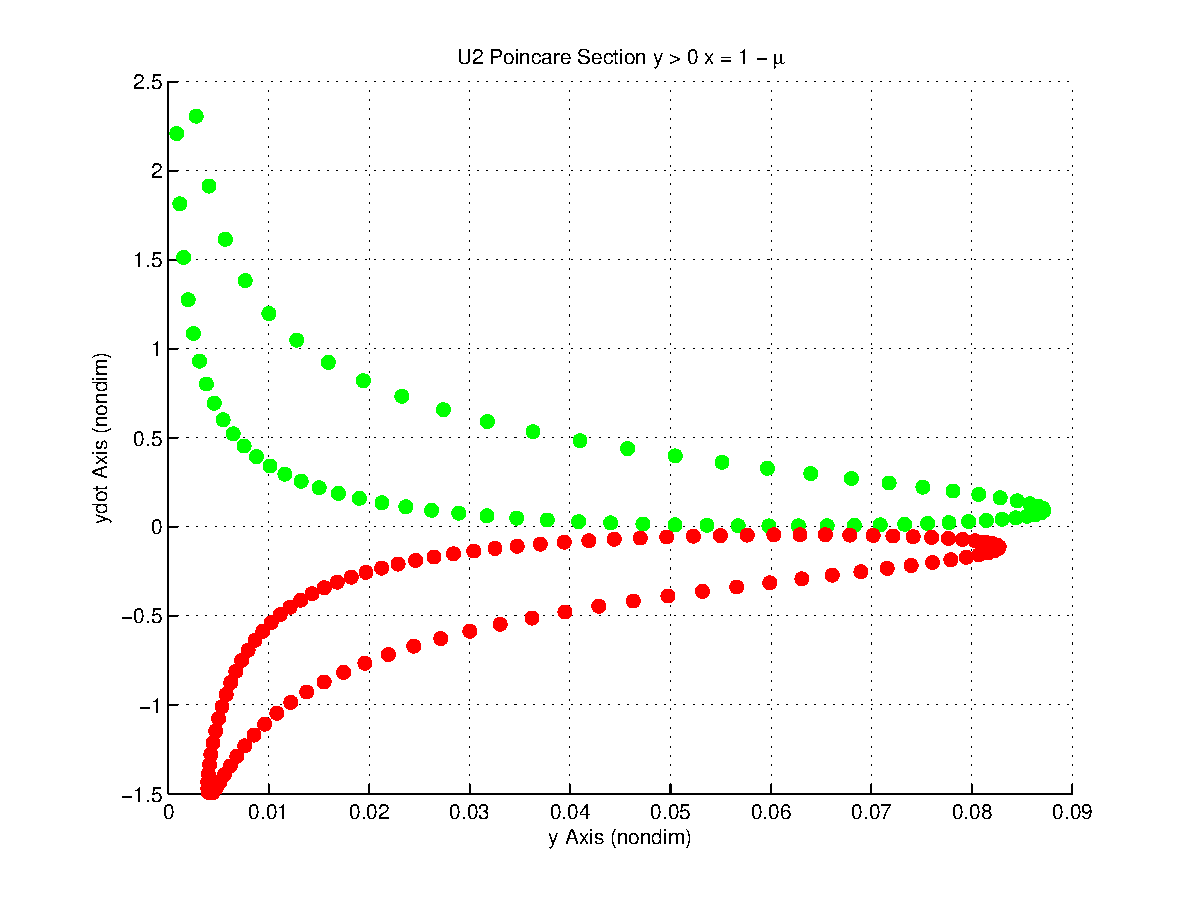
\includegraphics[width=0.5\columnwidth]{U2_poincare}
\end{figure}

	\pause
	\begin{itemize}
		\item Transfer is limited to intersecting regions
	\end{itemize}
	
	\note[itemize]{
		\item Lower state space from 4D to 2D
		\item Energy Constant and Poincar\'e section plane are two constraints which reduce the state space
		\item Extend invariant manifold transfer concept with addition of control input
	}
\end{frame}%--------------------------------%

